\section{Determination of $\nu_\mu$ Flux and Uncertainty at the Near Detector}
\label{sec:FluxDetermination}

Historically, uncertainties in the neutrino flux have been the largest source of systematic error in oscillation and cross section measurements. A primary goal in the construction of the ND280 complex was the reduction in the uncertainty in the expected neutrino flux at the Super-K far detector. For a cross section measurement made at ND280, we do not have the benefit of an additional neutrino interaction detector placed closer to the beam source. Regardless, a collection of data from external experiments, cutting-edge simulation techniques and measurements from many dedicated beam monitoring devices are used to predict the absolute neutrino flux and the related uncertainty at the near detector. We summarize some of the most relevant sources of error and the methodology behind the flux prediction without delving too far into the details of the external experiments and the monitoring equipment. All of the work in this Section was completed by the beam group of the T2K experiment and greater detail can be found in Ref~\cite{fluxpred} and Ref~\cite{fluxtn}.

In T2K, a primary beam of 30~GeV protons collides with a carbon target to produce secondary pions and kaons. These particles then decay into the proper neutrino flavors, yielding a flux of primarily $\nu_\mu$ at ND280. There are several steps involved in simulating this process. First, a common package called FLUKA is used to simulate the proton-carbon interactions and generate the secondary pion and kaon 4-vectors. Then JNuBeam, a GEANT based simulation package, is used to track the particles as they exit the thick carbon target. These secondaries are tracked to the decay volume downstream of the target where JNuBeam simulates neutrino production via decay. The neutrinos are the tracked to the ND280 complex and the absolute flux is calculated. Figure \ref{fig:fluxparent} shows a breakdown of the parent secondary particle responsible for the  $\nu_\mu$, anti-$\nu_\mu$, $\nu_e$ and anti-$\nu_e$ fluxes at ND280. We are primarily interested in the $\nu_\mu$ flux, though the other neutrino fluxes do slightly inflate our absolute flux error on the cross section measurement.

Several methods were used to tune the simulation to actual data. The most valuable tuning data comes from the NA61/SHINE collaboration, a T2K dedicated experiment. Data collected from 2007 to 2010 from the NA61/SHINE experiment is used. NA61/SHINE ran a 30~GeV proton beam on a graphite target to study proton-carbon interactions in the same energy regime as T2K. Both a thin target and a thick target were used. The thin target had a density of 1.84~g/cm$^3$ and was 2~cm thick while the thick target was a T2K target replica with a density of  1.83~g/cm$^3$, length of 90~cm and diameter of 2.6~cm. The simulation was compared to the collected data and only a few physics parameters were tuned to account for discrepancies. The tuned parameters are the 
secondary and tertiary pion production rates, the secondary and tertiary kaon production rates and the pion/kaon interaction rates.

\begin{figure}[h]
\centering
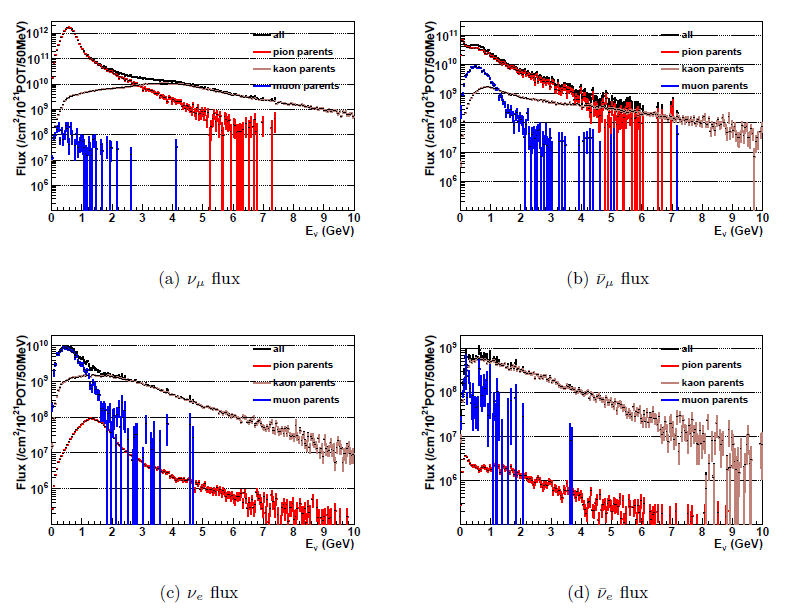
\includegraphics[width=6in]{Figures/flux/fluxparent.PNG}
\caption{A breakdown of the parent particle contribution to the production of $\nu_\mu$, anti-$\nu_\mu$, $\nu_e$ and anti-$\nu_e$ fluxes at ND280.} 
\label{fig:fluxparent}
\end{figure}

The secondary pion production rates are externally tuned to the NA61 thin target data. A ratio is calculated for each flux energy bin between the thin target pion multiplicity and the FLUKA simulated multiplicity. Tertiary pion production rates are similarly tuned by using NA61 data after scaling the data to lower nucleon energies. To tune the particle interaction rate, T2K uses results from non-dedicated experiments measuring hadronic cross sections on carbon and aluminium within the relevant energy regimes. The hadronic interaction simulation software GCALOR is used to calculate the hadronic interaction rate and any discrepancy with the selected external literature is corrected by a simple weighting scheme. The study found that the production rates within the target agreed well with pre-existing data, but interactions outside the graphite target required some tuning. The tuning scheme uses the suggested weighting scheme calulated as a function of distance traveled by different particle through different materials. Like the pion production tuning, the final result once the weights are applied are ratios of tuned flux to nominal flux in bins of energy. 

Secondary and tertiary kaon production rates were also studied and tuned. Secondary kaon production tuning is performed using data from NA61, Allaby {\it et al.} \cite{allabyref} and Eichten {\it et al.} \cite{eichtenref}. Kaons within the phase space studied by NA61 prioritize that NA61/SHINE data for calculating tuning ratios. Similarly, kaons in the phase space of the Allaby {\it et al.} and Eichten {\it et al.} experiments prioritize measurements from these two papers to calculate the tuning ratios. Tertiary kaon production is done by extrapolating between weights calculated from the three data sources of NA61, Allaby {\it et al.} and Eichten {\it et al.} The final results of the entire tuning procedure are shown in Figure \ref{fig:tuningresult}. The four plots show the tuning ratio vs. the flux energy for the four different neutrinos present in our beam. Again, we are primarily concerned with the $\nu_\mu$ flux. Also note that despite the large tuning ratios at high neutrino energies, the actual change in absolute flux is small as our beam is peaked at 600~MeV with very low flux at the higher energies.

\begin{figure}
\centering
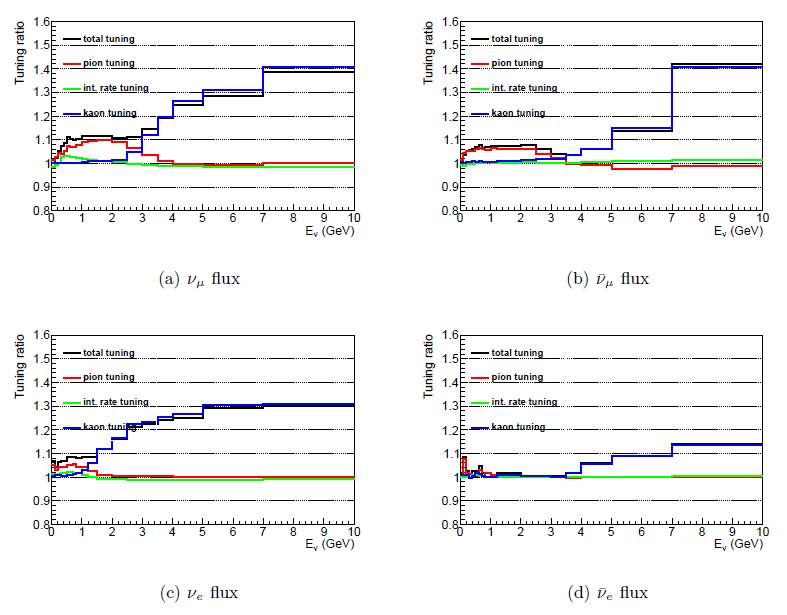
\includegraphics[width=6.5in]{Figures/flux/tuningresult.PNG}
\caption{The results of the tuning applied to pion and kaon production and interaction rates. The tuning is implemented as a ratio of the tuned value to the nominal simulation value plotted vs. neutrino energy. This ratios are shown in the plots for the  $\nu_\mu$, anti-$\nu_\mu$, $\nu_e$ and anti-$\nu_eu$ fluxes at ND280.} 
\label{fig:tuningresult}
\end{figure}

The tuning procedure predicts the absolute flux at ND280 and eventually yields the integrated flux we use to calculate the CC inclusive cross section. The last step is to evaluate the uncertainties on the predicted flux for propagation into our cross section measurement. As mentioned, this is one of the largest errors in historical cross section measurements and it is no different for our analysis. The sources of uncertainty in the absolute flux are:

\begin{itemize}
\item Kaon production multiplicity
\item Pion production multiplicity
\item Interaction rate (production cross section)
\item Secondary nucleon production
\item Off-axis angle
\item Proton beam
\item Horn field asymmetry
\item Horn angular alignment
\item MC statistics
\item Horn alignment
\item Target alignment
\end{itemize}

The list of sources can be broken into two overarching types of errors. The first four error sources are physics simulation errors and the remainder are instrumental and mechanical errors. The physics errors are derived directly from the data used to tune each of the parameters in the previous procedure. Specifically, the errors are:

\begin{itemize}
\item Propagations of the NA61, Eichten {\it et al.} and Allaby {\it et al.} errors through the flux tuning
\item Areas of production phase space not covered by any existing data
\item From the tuning procedure itself
\end{itemize}

Finally, as described in the beam construction section, there are many monitors responsible for measurement of mechanical parameters such as horn alignment, off axis angle, etc. The instrumental uncertainties in these monitoring devices are directly propagated via simulation to estimate the overall mechanical uncertainty in the flux. The total fractional flux uncertainty as well as the source-by-source breakdown of the fractional flux uncertainty for all four neutrino types is shown in Figure \ref{fig:fracuncertainty}. The fractional uncertainty is presented as a function of neutrino energy, and is used that way when propagating them into the cross section measurement later. Also, it is interesting to note that the total flux uncertainty is almost entirely from physics simulation parameters and not from mechanical and instrumental uncertainty of the T2K beam facility.

\begin{figure}
\centering
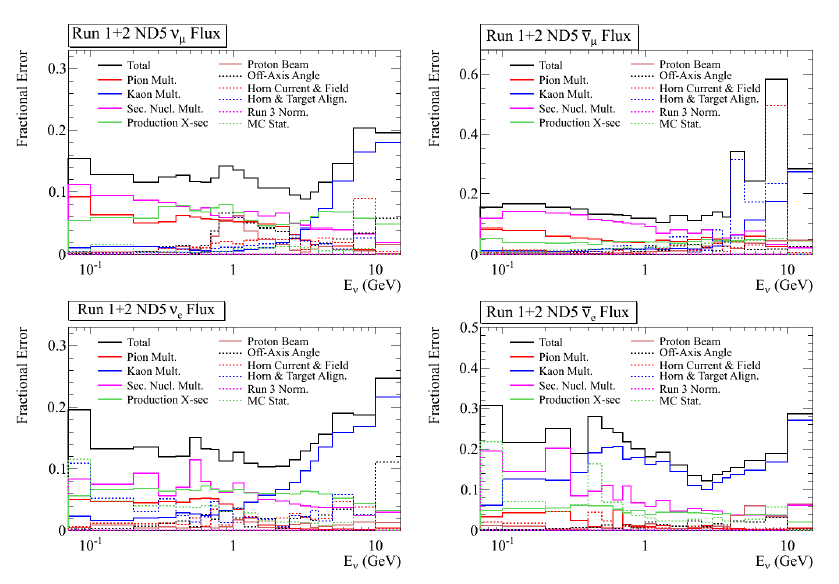
\includegraphics[width=6.5in]{Figures/flux/fracuncertainty.PNG}
\caption{The fractional error on each bin of flux energy broken down by error source.} 
\label{fig:fracuncertainty}
\end{figure}

\begin{figure}
\centering
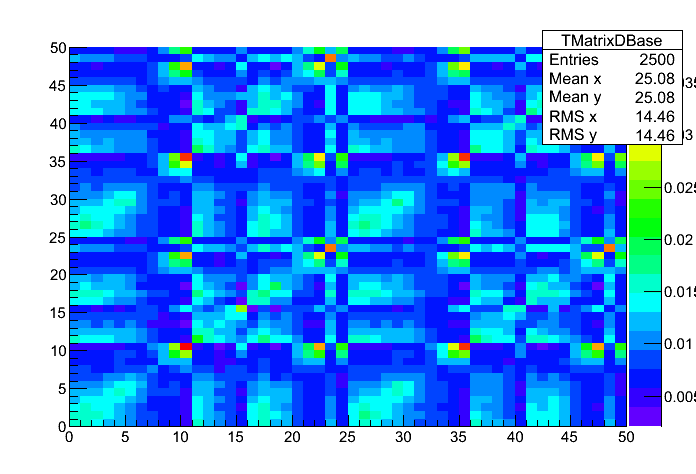
\includegraphics[width=6in]{Figures/flux_cov_init.png}
\caption{The flux covariance matrix. Only the ND280 bins corresponding to the 25~bin$\times$25~bin square at the bottom left are used.}
\label{fig:fluxcov}
\end{figure}

As errors in each bin of neutrino energy are correlated with errors in other bins, a covariance matrix is also produced and shown in Figure \ref{fig:fluxcov}. This flux covariance matrix is used directly in this analysis as well as other T2K measurements. Unlike the other plots in this section, the bins of the covariance matrix are not in units of neutrino energy. For the purposes of analysis, the flux uncertainty is parametrized by normalization factors on varying bins of neutrino energy. Each neutrino type and flavor has a different binning scheme used depending on its contribution to the total flux. The $\nu_\mu$ flux is divided into 11 bins, the anti-$\nu_\mu$ flux into 5 bins, the $\nu_e$ flux into 7 bins and the anti-$\nu_e$ flux into 2 bins. The bin limits used are as follows (in GeV):

\begin{itemize}
\item $\nu_\mu$: 0, 0.4, 0.5, 0.6, 0.7, 1.0, 1.5, 2.5, 3.5, 5.0, 7.0, 30.0
\item anti-$\nu_\mu$: 0, 0.7, 1.0, 1.5, 2.5, 30.0
\item $\nu_e$: 0, 0.5, 0.7, 0.8, 1.5, 2.5, 4.0, 30.0
\item anti-$\nu_e$: 0, 2.5, 30.0
\end{itemize}

The axes of the covariance matrix in Figure \ref{fig:fluxcov} follow the described binning scheme. From 0 to 25, the first set of bins are the $\nu_\mu$, anti-$\nu_\mu$, $\nu_e$ and anti-$\nu_e$ bins in that order. The second set of bins from 25 to 50 also follow the same order. The first set corresponds to the flux at ND280 and the second set to the flux at Super-K. As our analysis only uses data from the near detector, any entries outside the 0 to 25 bin range are neglected. However, note that in a full oscillation analysis, the ND280 vs. Super-K flux covariance cross terms are crucial in properly constraining the flux prediction at the far detector.